\chapter{GEP-NEAT}\label{chapter:gep_neat}
This chapter provides covers GEP-NEAT, a blend between NEAT (covered in Chapter \ref{sec:ne_neat}) and gene expression programming (covered in Chapter \ref{chapter:gep}). An introduction to GEP-NEAT is given in Section \ref{sec:gep_neat_introduction}. The proposed algorithm is explained in-depth in Section \ref{sec:gep_neat_proposed_algorithm}, after which the prototype implementation is discussed in Section \ref{sec:gep_neat_protoype_implementation}. Finally, the prototype is applied to a few problems to benchmark the algorithm's performance in Section \ref{sec:gep_neat_model_validation}.

\section{Introduction}\label{sec:gep_neat_introduction}
Neuroevolution (Chapter \ref{chapter:neuroevolution}) focuses on finding creative ways to optimize artificial neural networks (ANNs) using evolutionary algorithms (Chapter \ref{chapter_ea}). Unlike the traditional methods such as backpropagation and gradient descent to train neural networks, neuroevolution leverages Darwinian principles to evolve the topology of the neural network along with its weights and biases. NEAT, as explained in Chapter (\ref{sec:ne_neat}), is a powerful method to evolve both the structure and weights of a neural network. One of the most significant challenges NEAT faces is its computational cost due to the topological sort needed when evaluating a neural network sample. In other words, not only is the mapping between the genotype and phenotype a challenging task to overcome, but the forward feeding of values to calculate fitness an expensive task. \bigskip

\noindent GEP, and its extension GEP-NN, is an evolutionary algoirthm that combines the genetic algorithms with the powerful representation of genetic programming to solve complex problems, especially tasks that require a non-linear structure such as trees, graphs, etc. GEP's novelty lies in the genotype-phenotype mapping of a chromosome using Karva notation. \bigskip

\noindent GEP-NN, the proposed algorithm, takes inspiration from the expressive power in chromosome representation that GEP provides, and the core principles of NEAT. Among this, GEP-NN adds additional novelty by reconstructing the representation of innovation numbers that NEAT employs. Using the concept of a meme by Richard Dawkins, a new selection and mutation operators are introduced that takes advantage of the innovation numbers which tracks sub-configurations. Additionally, GEP-NN bridges the gap in bias introduction that the original GEP-NN missed and introduces a mechanism on how to embed bias information within the chromosome.

\section{Proposed Algorithm}\label{sec:gep_neat_proposed_algorithm}
\subsection{Evolutionary Life Cycle}
The aim og GEP-NEAT is to combine the expressive power of Karva notation within GEP which ensures syntactically correct programs with the neuroevolutionary principles of NEAT to effectively speciate and evolve an evolutionary population. To begin, both NEAT and GEP both have commonalities of a generic evolutionary flow, that is, create an initial population, represent the chromosome adaquitely, evalute each chromosome's fitness, decide whether to terminate the process and if not, apply genetic operators and repeat the process until the stop conditions are met. Differences lie however in relation to the novelties that each one presents. For example, in NEAT, speciation is encompassed within the evolutionary cycle whereby the historical genes for each generation is tracked in a lookup table by means of an innovation number. This innovation number table is referenced when calculating a compatabiliyt distance in order to speciate chromosomes so that they compete within their own niches (\cite{stanley2002evolving}). GEP on the other hand, orignally follows the basic genetic algorithm flow, however, introduces an abundandt amount of genetic operators to introduce diversity within the genetic pool and allow manifestations of reproducible building blocks to be used within genetic structures (\cite{ferreira2006gene}). GEP-NEAT takes inspiration from both these algorithms to form the framework that is seen in Figure \ref{fig:gep_neat_framework}. \bigskip

\noindent There are commonalities that GEP-NEAT shares with NEAT and GEP-NN, such as the intial stages of creating an intial population and calculating fitness. Futhermore, speciation is insired from NEAT and likewise, the specific genetic operators is inspired from GEP. Steps such as the calculation of innovatyion and meme influence are specfic to GEP-NEAT. In order to properly understand the intracacies of the evolutionary framework depicited in Figure \ref{fig:gep_neat_framework}, it is best to explain from start to finish incrementally.

\begin{figure}[H] % Use [H] to suppress floating and place the figure/table exactly where it is specified in the text
	\centering % Horizontally center the figure on the page
	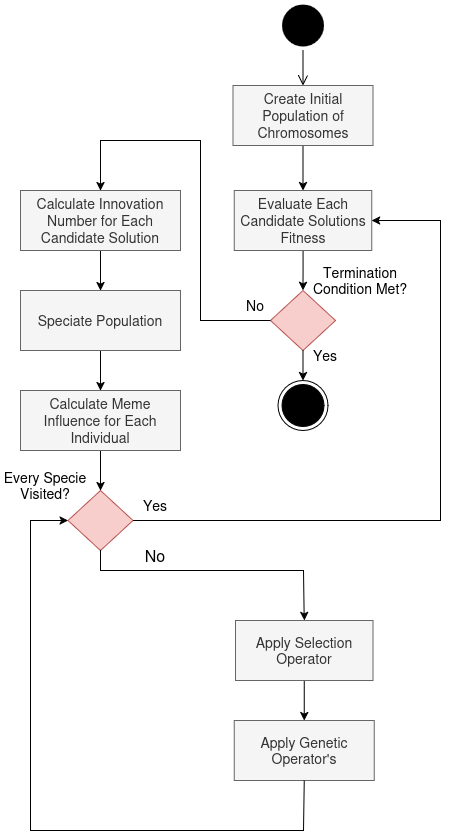
\includegraphics[width=0.65\textwidth]{Figures/chapter_gep_neat/gep_neat_framework.png} % Include the figure image
	\caption{Evolutionary Lifecycle of GEP-NEAT}
	\label{fig:gep_neat_framework} % Unique label used for referencing the figure in-text
\end{figure}

\subsection{Representation}\label{sec:gep_neat_representation}
NEAT-GEP takes inspiration from the genotype-phenotype mapping that GEP introduces, that is, using Karva notation. There are a few changes amended to the representation, with the fist being the tree style encoding. In traditional GEP, k-expressions are converted to expression trees by reading from left-to-right and top-to-bottom. Seeing that conversion is required to evaluate the expression  tree to calculate fitness, encoding the expression tree in this manner can lead to computational strain during the evolutionary process for large populations and complex linear strings. Mentioned in Chapter \ref{chapter:gep}, otherway of encoding these linear strings include prefix and postfix. P-GEP which embeds linear strings in postfix fashion. In doing so, the traditional GEP genetic operators are more proective for subscrutres which aids in more powerful search capabilities. To illustrate this, Figure \ref{fig:gep_neat_p_gep} shows how the standard karva notation differs from prefix notation with the different subtree configurations highlighted in purple, blue and green. Evidently, when genetic operations are applied to standard karva notation, these subtree configurations are lost, however, when applied to prefix notation, it can preserve subtree configurations. An example of this is when single point crossover is applied with the crossover point between gene 3 and 4.

\begin{figure}[H] % Use [H] to suppress floating and place the figure/table exactly where it is specified in the text
	\centering % Horizontally center the figure on the page
	\includesvg[width=0.80\textwidth]{Figures/chapter_gep_neat/gep_neat_p_gep.svg} % Include the figure image
	\caption{GEP Encoding Scheme versus P-GEP Encoding Scheme}
	\label{fig:gep_neat_p_gep} % Unique label used for referencing the figure in-text
\end{figure}

\noindent To best explain how GEP-NEAT chromsoome work, an abritary example will be used throughout the Chapter. Consider a linear string that has a head size of $3$ and a maximum function symbol arity of $3$ with the following arbitrary functions set ${D, T}$ and terminal set ${a, b, c}$. Function symbol $D$ takes 2 inputs while $T$ takes 3. The corresponding tail size would be: $t = h \times (n_{max} - 1) + 1 = 3 \times (3 - 1) + 1 = 7$. A candiate solution would then have length $genome \:\: length = h + t = 2 + 7 = 9$. In the original GEP paper, both a weight and threshold domain was encoded in the linear string. Although a threshold domain is useful in neural networks with simple activation functions such as binary step, they can be quite limiting. For this reason, only a weight domain is encoded in the linear string. The linear string in reference has a weight domain length of $D_w = h \times n_{max} = 3 \times 3 = 9$. A lookup weight array which the weigh values serve as indices and pulls from the weight array may look as follows of size 5: $[-1.2,\:2.3,\:3.2,\:4.4,\:-0.5,\:6.0]$. A sample chromosome may looks follows:

\begin{equation}\label{example:representation}
    \begin{array}{cccccccccccccccccc}
        0 & 1 & 2 & 3 & 4 & 5 & 6 & 7 & 8 & 9 & 0 & 1 & 2 & 3 & 4 & 5 & 6 & 7 \\
        D & a & T & a & b & c & a & b & a & 5 & 2 & 4 & 1 & 2 & 3 & 3 & 2 & 6
    \end{array}
\end{equation}

\noindent To reiterate, gene 0 to 5 represents the actual expression tree while gene 6 to 8 are buffer symbols. Another short fall of GEP-NN, is that bias nodes do not exist in the implementation. The original research on GEP-NN was applied to problems that was not necessarily impacted significantly by the lack of biasing with the neural network, however, with solution spaces that are much larger, biasing proves to be a much more essential component to avoid performance issues. Therefore, there will be an ammendment to the original GEP-NN algorithm as the first \textbf{novelty} mentioned. In order to encapsulate a biasing within the expression tree, every function symbol will enscapsulate two things:

\begin{itemize}
    \item \textit{bias enabled} - this stores a boolean value to determine whether a bias is enabled on the function symbol
    \item \textit{bias weight} - this stores the bias weight
\end{itemize}


\noindent To continue with the example, consider the function symbols in the expression string of Equation \ref{example:representation} to have the following bias information:
\begin{itemize}
    \item $D$
    \begin{itemize}
        \item \textit{bias enabled}: \textbf{true}
        \item \textit{bias weight}: \textbf{0.4}
    \end{itemize}

    \item $T$
    \begin{itemize}
        \item \textit{bias enabled}: \textbf{false}
        \item \textit{bias weight}: \textbf{2.3}
    \end{itemize}
\end{itemize}


\noindent This candidate solution represents the expression tree and in turn neural network seen in Figure \ref{fig:gep_neat_representation_example_tree}. Just as forward feeding in a traditional neural network works, values are fed into $a$, $b$, $c$ and the expression tree is evaluated in order to obtain the neural network output.

\begin{figure}[H] % Use [H] to suppress floating and place the figure/table exactly where it is specified in the text
	\centering % Horizontally center the figure on the page
	\includesvg[width=0.8\textwidth]{Figures/chapter_gep_neat/gep_neat_representation_example_tree.svg} % Include the figure image
	\caption{Example GEP-NEAT Candidate Solution Expression Tree of Linear String in Equation \ref{example:representation}}
	\label{fig:gep_neat_representation_example_tree} % Unique label used for referencing the figure in-text
\end{figure}

\noindent With reference to Figure \ref{fig:gep_neat_representation_example_tree}, the expression tree representation is decoded from the linear string using prefix notation. Although it will be later explained, the weight domain values are assigned in a fashion of depth first and works it way up, in a similar way that that symbolic regression trees get evaluates. In addition to this, each weight value corresponds to its index in the weight lookup array. Lastly, as mentioned, each function symbol has a bias node attached with D having its bias enabled and T having its bias disabled. \bigskip

\noindent Another shortfall the original GEP-NN algorithm had was its limitation in activation functions used. As mentioned, a threshold domain was used for each function symbol and had neuron's output 0 when the weighted sum was below that respective input and 1 otherwise representing a binary step function essentially. In the orignal GEP (and its extension GEP-NN), the only weighted sum functions used was of a linear nature, that is, having 3 function symbols, $D$, $T$, and $Q$, with function arity 2, 3, and 4 respectively. It was proved that the standard version of GEP-NN could not solve symbolic regression and classification problems, however, with the symbols modified such that it could represent the subtraction, multiplication, and division operator, it could overcome this limitation (\cite{improvedGepnn}). This however still not addressed more powerful trasnfer fucntion calculations that traditional neural networks provide. For this reason, the algorithm introduces as the next \textbf{novelty} different activaton functions. At each function symbol, the weighted sum is calcualted, that is,  the addition of all inputs plus the bias. Each function symbol will then encode its own activation function that is applied to this transfer function result. The function set is configurable in the sense that different functiion symbols with different arities is added, each with their own acitvation fucntion. THe idea is that, just as a neural netwrok is designed to make use of particular activation functions, so will GEP-NEAT. In addition to this, the function set cna also be configured to inclulde a wide range of activation function each with different function arities so that the algorithm can \textit{learn} which activation functions to use.


\subsection{Initial Population}
In the original GEP algorithm, Candida mentions that in order to speed up the evolutionary process of finding a suitable candidate, a start-protocol is employed which is that the an intial population is generated until a viable solution is find such that the fitness is not minimum. The purpose of this from GEP's persepctive is that every offspring is part of a lineage from a sole founder as a means to accelerate the exploitation vs exploration scheme \cite{ferreira2006gene}. The obvious implication of this is that there runs a risk of candidate solutions stagnating around local optima. \bigskip

\noindent In the case of NEAT, the concept of starting out minimally is introduced. NEAT does this by generating a population such that there are no hidden nodes forcing the resulting structures to be as minimal as possible. In doing so, the idea is that structural innovations are intended which means that solutions in the lowest dimentional space is searched for which leads to performance gains (\cite{stanley2002evolving}). Mentioned in the original paper of NEAT, typical algorithms don't do this because they run the risk of topological innovations being prematurely killed. NEAT solves this by protecting structural innovations through historical gene tracking by means of innovation numbers. \bigskip

\noindent GEP-NEAT does not inherit the start-up control mechanism that GEP makes use of in order to mitigate the chance that candiate solutions may prematurley stangate around local optima. Instead, GEP-NEAT adapts the \textit{starting out minimally} dependency compoennt NEAT mentions by generating individuals that have only one function symbol which is in the root of the linear chromosome during the intialisation phase. An example of this, is the linear string shown in Equation \ref{example:gep_neat_initial}, and its phentotype representation shown in Figure \ref{fig:gep_neat_initial_example}.

\begin{equation}\label{example:gep_neat_initial}
    \begin{array}{cccccccccccccccccc}
        0 & 1 & 2 & 3 & 4 & 5 & 6 & 7 & 8 & 9 & 0 & 1 & 2 & 3 & 4 & 5 & 6 & 7 \\
        D & a & b & a & b & c & a & b & a & 5 & 2 & 4 & 1 & 2 & 3 & 3 & 2 & 6
    \end{array}
\end{equation}

\begin{figure}[H] % Use [H] to suppress floating and place the figure/table exactly where it is specified in the text
	\centering % Horizontally center the figure on the page
	\includesvg[width=0.6\textwidth]{Figures/chapter_gep_neat/gep_neat_initial_example.svg} % Include the figure image
	\caption{Example GEP-NEAT Candidate Solution Expression Tree of Linear String in Equation \ref{example:representation} Generated Through Initialisation Phase}
	\label{fig:gep_neat_initial_example} % Unique label used for referencing the figure in-text
\end{figure}

\noindent In doing so, the initial population generated all have genotypes that represent networks with only a single input and output layer (no hidden layer). This aligns with the reasoning NEAT imposes whereby structural innovations are intended and the simplest solution space is explored first.


\subsection{Evaluating Candidate Solutions}
Section \ref{sec:gep_neat_representation} details how candidate solutions represent linear strings in their genotype form and translate using prefix notation into the respective expression tree (neural networks). Converting between genotype and phenotype for complex lienar strings and iteratively over many generations can incur expensive computational efforts. \bigskip

\noindent S\_GEP, an extension of P-GEP has the added benefit of evaluating the expression string without the need to convert it to an expression tree. Although there is no research on its use in GEP-NN, the idea to encorate it in GEP-NEAT is that forward feeding values in an expression tree already involves computationally expensive operations, so this would greatly benefit the calculations of fitness when doing this repeatedly throughout many candidate solution samples over many generations. Although S\_GEP was premis was covered in Chapter \ref{sec:gep_current_research}, with the added concept of proper activation functions and biases, the algorithm is changed slightly. Firstly, in order to evaluate the expression tree, values are replaced with the terminal values so that mathematic operation can commence. For example, if the network is being evolved to solve the XOR problem, then their would be 4 test values that would need to be fed into the network, that being, 00, 01, 10, and 11. For each case, the inputs would replace terminal symbols, so for example, a would be the first digit and b the second. The next step would be that the effective gene length is required in order to know what part of the linear string is the coding region. This is calculated using Algorithm \ref{alg:gep_neat_el}.

\begin{algorithm}
	\caption{Effective gene length (adapted from \cite{peng2014improved})}\label{alg:gep_neat_el}
	\begin{algorithmic}[1]
	% \Ensure $y = x^n$
	\item \textbf{Input}: String of gene symbols
	\item \textbf{Output}: eL
	\item Initialize variables $Len=1$ and $count=0$
	\item \textbf{while} scanning gene symbols starting from left to right:
	\item \quad $Len = Len + 1$;
	\item \quad \textbf{if} current gene symbol is function:
	\item \quad \quad $count = count - 1$
	\item \quad \textbf{else}:
	\item \quad \quad $count = count - 1$
	\item \quad \textbf{if} $count < 0$:
	\item \quad \quad return $eL=Len$ as output
\end{algorithmic}
\end{algorithm}

\noindent Once the effective gene length is known, the linear string can be evaluated using the concept of polish notation as the encoding has been done in prefix notation. The linear string is evaluated using Algorithm \ref{alg:gep_neat_evaluate}.

\begin{algorithm}
	\caption{GEP-NEAT Evaluation Algorithm (inspired from \cite{peng2014improved})}\label{alg:gep_neat_evaluate}
	\begin{algorithmic}[1]
	\item Calculate eL using Algorithm \ref{alg:gep_neat_el}
	\item set \textit{stack} array variable to an empty list
	\item set \textit{weight\_index} variable to 0
	\item \textbf{while} reading effective gene from right to left using eL:
	\item \quad \textbf{if} current gene is a terminal symbol:
	\item \quad \quad push terminal symbol on stack
	\item \quad \textbf{else if} current gene is function symbol:
	\item \quad \quad set \textit{weighted\_sum} variable to 0
	\item \quad \quad \textbf{for} number of function symbol inputs:
	\item \quad \quad \quad pop value from stack and multiply with weight from weight lookup array at index \textit{weight\_index}
	\item \quad \quad \quad add result value to \textit{weighted\_sum}
	\item \quad \quad \quad increment \textit{weight\_index} by 1
	\item \quad \quad \textbf{if} bias is enabled for current function symbol:
	\item \quad \quad \quad add function symbol's bias value to \textit{weighted\_sum}
	\item \quad \quad apply function symbol's activation function to \textit{weighted\_sum}
	\item \quad \quad push result value onto stack
	\item pull value from stack and return
\end{algorithmic}
\end{algorithm}

\noindent Once the linear string is evaluated, it is then fed into a fitness function to calculate a fitness value. Fitness functions are problem specific, for example, in both NEAT and GEP, the XOR uses the folloiwng fitness function:

\begin{equation}\label{alg:absolute_error}
    f_{i} = \sum_{j=1}^{C_t}(M-|C_{(i,j)}-T_{(j)}|
\end{equation}

\noindent where:
\begin{itemize}
    \item $f_i$ is fitness for candidate solution $i$
    \item $C_t$ is the number of test cases
    \item $M$ is the maximum value for a fitness case
    \item $C_{(i,j)}$ is the value returned by individual $i$ for case $j$
    \item $T_{(j)}$ is the target value for case $j$
\end{itemize}

\noindent Other problems such as the cartpole problem have fitness functions based on a reward scheme whereby for every episode thta the cartpole balances the pole, it receives an abritary incentive reward value and otherwise, a zero value.

\subsection{Speciation}
The next step of the algorithm is to do two things, that is, calculate innovation numbers and speciate. NEAT uses innovation numbers to track the historical lineage of genes to in order to preserve innovation, in particular, innovative structures. NEAT assigns innovation numbers by keeping track of a global table and whenever an new, unseen connection between two nodes appear, the global innovation number is incremented. Innovation numbers in this was as seen in Chapter \ref{sec:ne_neat} allows two chromosomes to be compared by calculating how the difference in number of innovation numbers they share and further allows speciation. \bigskip

\noindent GEP-NEAT adopts the concept of innovation numbers by redefining what they represent. Innovation numbers are redefined to represent sub-tree information. In other words, each subtree represents a unique innovation number. Subtree can then reference reference other innovation numbers. To visually illustrate, refer to Figure \ref{fig:gep_neat_innovation_number}. The tree is traversed in the same manner when evaluating the expression tree. As values are popped onto the stack, each subtree is analysed and checked against a global innovation number lookup table. If the subtree exists in the lookup table, that innovation number is used, otherwise, the subtree is added to the lookup table as a new entry and incremented innovation number value. Algorithm \ref{alg:gep_neat_innovation_number} shows this mechanism.

\begin{figure}[H] % Use [H] to suppress floating and place the figure/table exactly where it is specified in the text
	\centering % Horizontally center the figure on the page
	\includesvg[width=\textwidth]{Figures/chapter_gep_neat/gep_neat_innovation_number.svg} % Include the figure image
	\caption{Innovation Number Assignment on GEP-NEAT Expression Tree}
	\label{fig:gep_neat_innovation_number} % Unique label used for referencing the figure in-text
\end{figure}

\begin{algorithm}
	\caption{GEP-NEAT Innovation Number Algorithm}\label{alg:gep_neat_innovation_number}
	\begin{algorithmic}[1]
	\item Calculate eL using Algorithm \ref{alg:gep_neat_el}
	\item set \textit{stack} array variable to an empty list
	\item \textbf{while} reading effective gene from right to left using eL:
	\item \quad \textbf{if} current gene is a terminal symbol:
	\item \quad \quad push terminal symbol on stack
	\item \quad \textbf{else if} current gene is function symbol:
	\item \quad \quad push current function symbol to stack
	\item \quad \quad access index [function symbol's arity plus 1] from stack to get subtree
	\item \quad \quad set \textit{innovation\_number} variable to 0
	\item \quad \quad \textbf{if} innovation number does not exist in lookup table:
	\item \quad \quad \quad set \textit{innovation\_number}  to length of lookup table minus 1
	\item \quad \quad \textbf{else}:
	\item \quad \quad \quad set \textit{innovation\_number} variable to found value in lookup table
	\item \quad \quad push \textit{innovation\_number} to stack
\end{algorithmic}
\end{algorithm}

\noindent Innovation numbers serves as a system to represent subtree configuration, which in turn can be used to represent entire expression trees. Every expression tree in this regard can be expressed using its \textit{innovation number composition} which is a list comprising of innovation number that make up their tree. Each innovation number with that composition list stores the subtree that the innovation number represents with its respective weights. This would mean that this composition list is keyed on the innovation number with its value being the a tuple representing its subtree and weight respective weights. The \textit{innovation number composition} is calculated using Algorithm \ref{alg:gep_neat_innovation_number_composition}. For example, the \textit{innovation number composition} for the expression tree seen in Figure \ref{fig:gep_neat_innovation_number} has the corresponding \textit{innovation number composition} seen in Figure \ref{fig:gep_neat_innovation_number_composition}.

\begin{algorithm}
	\caption{GEP-NEAT Innovation Number Composition Algorithm}\label{alg:gep_neat_innovation_number_composition}
	\begin{algorithmic}[1]
	\item Calculate eL using Algorithm \ref{alg:gep_neat_el}
	\item set \textit{weight\_index} variable to 0
	\item set \textit{stack} array variable to an empty list
	\item \textbf{while} reading effective gene from right to left using eL:
	\item \quad \textbf{if} current gene is a terminal symbol:
	\item \quad \quad push terminal symbol on stack
	\item \quad \textbf{else if} current gene is function symbol:
	\item \quad \quad set \textit{weights} array variable to empty list
	\item \quad \quad \textbf{for} number of function symbol inputs:
	\item \quad \quad \quad retrieve value from weight lookup array indexed at current input and add to weight array
	\item \quad \quad \quad increment \textit{weight\_index} by 1
	\item \quad \quad append  current symbol to stack
	\item \quad \quad access index [function symbol's arity plus 1] from stack to get subtree
	\item \quad \quad get innovation number using subtree from lookup table
	\item \quad \quad append innovation number with its corresponding subtree and \textit{weights} to the \textit{innovation\_number\_composition}
	\item \quad \quad push result value onto stack
	\item return \textit{innovation\_number\_composition}
\end{algorithmic}
\end{algorithm}

\begin{figure}[H] % Use [H] to suppress floating and place the figure/table exactly where it is specified in the text
	\centering % Horizontally center the figure on the page
	\includesvg[width=\textwidth]{Figures/chapter_gep_neat/gep_neat_innovation_number_composition.svg} % Include the figure image
	\caption{Innovation Number Composition Expression Tree in Figure \ref{fig:gep_neat_innovation_number}}
	\label{fig:gep_neat_innovation_number_composition} % Unique label used for referencing the figure in-text
\end{figure}

\noindent Similarly to how NEAT can represent a candidate solution entirely in terms of its innovation numbers, so can GEP-NEAT. GEP-NEAT adopts the same speciation mechanism as NEAT, that is, using a compatibility distance function. Inspired from NEAT, GEP-NEAT introduces the following compatibility distance function:

\begin{equation}\label{alg:speciation}
    \delta = \frac{c_1NM}{N} + c_2\cdot{\overline{W}}
\end{equation}

\noindent where:
\begin{itemize}
    \item $\delta$ is the compatibility distance between a pair of genomes
    \item $NM$ is the number of non-matching genes
    \item $\overline{W}$ is the average weight difference of matching gene arrays
    \item $N$ is the number of genes in the larger genome (serving as a normalization)
    \item $c_1$ and $c_2$ serve as adjustments in the importance of the two factors
\end{itemize}

\noindent In the original NEAT paper, although disjoint and excess genes were defined distinctively as two different components, they had no unique implication  as whole. For this reason, GEP-NEAT recognizes matching and non-matching genes. On this note, the average weight works slightly differently. Two genes representing the same subtree configuration can have different weights assosiated between the same connections, hence, in order to calculate the average weight difference:

\begin{equation}\label{alg:weight_difference}
    \overline{W} = \frac{\sum_{j=0}^{N}|W_{aj} - W_{bj}|}{N}
\end{equation}

\noindent where:
\begin{itemize}
	\item $\overline{W}$ is the average weight difference of the subtree
	\item $N$ is the number of child nodes in the subtree
	\item $W_{aj}$ is the weight of subtree '$a$' of child node $j$
	\item $W_{bj}$ is the weight of subtree '$b$' of child node $j$
\end{itemize} 

\noindent The number of matching and non-matching genes can then be calculated easily by converting an expression tree to its \textit{innovation number composition} counterpart, and analysing which genes are in common and which are not. Figure \ref{fig:gep_neat_innovation_number_compare} shows that the matching genes between expression tree 1 and 2 are $\{2\}$, and the non-matching genes are $\{1, 3, 4, 5\}$.

\begin{figure}[H] % Use [H] to suppress floating and place the figure/table exactly where it is specified in the text
	\centering % Horizontally center the figure on the page
	\includesvg[width=\textwidth]{Figures/chapter_gep_neat/gep_neat_innovation_number_compare.svg} % Include the figure image
	\caption{Comparing Expression Trees Using Innovation Number Compositions}
	\label{fig:gep_neat_innovation_number_compare} % Unique label used for referencing the figure in-text
\end{figure}

\noindent Speciation occurs within every evolutionary generation by speciating individuals and follows algorithm \ref{alg:speciation_2}. Essentially, during each generation, the population is shuffled to give every individual an opportunity to be the representative individual of a species (in an attempt to better group individuals in species group). Every individual is then evaluated against every specie's representative individual and provided its compatibility distance is less than the compatibility threshold $\delta_{ct}$, it will then belong to that species. This process continues until every individual is part of a specie group.

\begin{algorithm}
	\caption{GEP-NEAT Speciation Algorithm}\label{alg:speciation_2}
	\begin{algorithmic}[1]
	\item Initialise empty list of \textit{species}
	\item Shuffle the population
	\item \textbf{for} every individual in population:
	\item \quad \textbf{if} species is empty:
	\item \quad \quad add individual as first specie group
	\item \quad \textbf{else}:
	\item \quad \quad \textbf{for} every specie in the \textit{species} list:
	\item \quad \quad \quad calculate compatibility distance between representative individual in current specie and current individual
	\item \quad \quad \quad \textbf{if} compatibility distance is less than compatibility threshold $\delta_{ct}$:
	\item \quad \quad \quad \quad add individual to current specie
	\item \quad \quad \quad \quad \textbf{break} to next individual
\end{algorithmic}
\end{algorithm}

\subsection{Meme Influence}
Richard Dawkins is a British evolutionary biologist and best known for his gene-centered view of evolutionary, most famously in his 1976 book \textit{The Selfish Gene}. In this book, Dawkins argues that genes are the primary units of natural selection, driving evolution through replication and competition (\cite{dawkins1981selfish}). Dawkins introduces the term "\textbf{meme}" in the \textit{The Selfish Gene} as a cultural analog to biological genes. A meme is a unit of cultural information such as an idea, behavior, or trend, that spreads from person to person via imitation. Importantly, memes are subject to variation, competition and selection, much like genes that drives evolution. \bigskip

\noindent Seeing that subtree configurations are tracked by means of  an innovation lookup table throughout the evolutionary cycle, GEP-NEAT takes advantage of this by introducing a new concept called the \textit{meme influence}. The \textit{meme influence} and \textit{innovation number contribution} are two additional attributes tracked within each innovation number and is used to rank sub-tree configurations. This attribute is calculated as shown in Algorithm \ref{alg:meme_influence}. The algorithm works by first calculating what each innovation numbers contribution is with regard to the individuals adjusted fitness (to the specie it belongs to). This is done using Equation \ref{equation:innovation_contribution}. The \textit{innovation contribution} value is then added to the result stored in every innovation number that makes up the individual's innovation number contribution. In doing this, information is being built up to describe which innovation numbers have contributed to the highest fitness according to adjusted fitness within each specie. Equation \ref{equation:innovation_contribution} assumes that each innovation number contributes equally to the success of a candidate individual, however, by tracking and incrementing each innovation numbers contribution collectively by all individuals within the population, innovation numbers that generally form part of higher fit individuals will tend to have higher innovation contributions. After the innovation contribution for every innovation number has been updated, the next step is to normalize these innovation contribution values so that they can be represented in a way that they can be ranked. Each innovation contribution value is then normalised according to Equation \ref{equation:normalise}. With the normalised value calculated, the meme influence value of individual $i$ is calculated using Equation \ref{equation:meme_influence} where $\alpha$ is the decay rate. The meme influence is calculated using a shifting average moving function in order to encourage current trends for a period of time until it fades away (\cite{haynes2012exponential}). The outcome of the meme influence calculation is to provide a mechanism in which innovation numbers can be ranked within every generation.

\begin{algorithm}
	\caption{GEP-NEAT Meme Influence Algorithm}\label{alg:meme_influence}
	\begin{algorithmic}[1]
	\item \textbf{for} specie in species:
	\item \quad \textbf{for} individual in specie:
	\item \quad \quad calculate \textit{innovation contribution} using Equation \ref{equation:innovation_contribution}
	\item \quad \quad \textbf{for} each innovation number in the current individual's innovation number composition:
	\item \quad \quad \quad innovation\_lookup\_table[innovation number][innovation contribution attribute] += \textit{innovation contribution}
	
	\item 

	\item \textbf{for} each innovation number in innovation\_lookup\_table:
	\item \quad calculate the normalised value for the current innovation number using Equation \ref{equation:normalise}
	\item \quad calculate innovation number contribution using Equation \ref{equation:innovation_contribution}
	\item \quad calculate the \textit{meme influence} for the current individual using Equation \ref{equation:meme_influence}
	\item \quad append the \textit{meme influence} value as attribute to the current innovation number
\end{algorithmic}
\end{algorithm}

\begin{equation}\label{equation:innovation_contribution}
    innovation\:contribution = \frac{individual\:adjusted\:fitness}{length(individual\:innovation\:number\:composition)}
\end{equation}

\begin{equation}\label{equation:normalise}
    normalised\:value_i = \frac{innovation\:contribution_i - min\:innovation\:contribution}{max\:innovation\:contribution - min\:innovation\:contribution}
\end{equation}

\begin{equation}\label{equation:meme_influence}
    meme\:influence_i = (\alpha \times normalised\:value) + ((1 - \alpha) \times meme\:influence_i)
\end{equation}

\subsection{Selection}
Both GEP and NEAT make use of well studied selection operators; NEAT uses tournament selection while GEP makes use of roulette wheel selection. The problem with this kind of selection mechanism is that the only information that the selection operator makes use of is fitness and has no strong relation to the innovation of structures that make up an individual. GEP-NEAT tracks a metric known as the \textit{meme influence} as an additional attribute alongside each innovation number giving a way in which innovation numbers can be ranked. GEP-NEAT introduces a new selection operator called \textit{Meme Influence Roulette Wheel Selection (MIRWS)} which is based on roulette wheel selection with the difference being that the \textit{meme influence} values are used as opposed to raw fitness scores of individuals. The new adjusted fitness scores based on the \textit{meme influence} values are calculated using Algorithm \ref{alg:mirws} and thereafter follows the generic roulette wheel based selection algorithm.

\begin{algorithm}
	\caption{GEP-NEAT Meme Influence Roulette Wheel Selection Algorithm}\label{alg:mirws}
	\begin{algorithmic}[1]
	\item \textbf{for} each individual in the population:
	\item \quad initialise \textit{total\_individual\_fitness} variable to 0
	\item \quad \textbf{for} each innovation number in the current individual's innovation number composition:
	\item \quad \quad \textit{total\_individual\_fitness} += current innovation numbers meme influence value
	\item \quad set the current individuals adjusted fitness to the \textit{total\_individual\_fitness}
	\item
	\item intialise \textit{selected\_individual} array to empty list
	\item \textbf{for} number of individuals required:
	\item \quad choose a random number between 0 and the total adjusted fitness based on the meme influence value
	\item \quad set \textit{current} variable to 0
	\item \quad \textbf{for} every individual in the population:
	\item \quad \quad \textit{current} += current individuals adjusted fitness
	\item \quad \quad \textbf{if} \textit{current} >= random number chosen:
	\item \quad \quad \quad append current individual to \textit{selected\_individual} list
	\item \textbf{return} \textit{selected\_individual}
\end{algorithmic}
\end{algorithm}

\subsection{Genetic Operators}
Once individuals are selected within every specie during every generation of the evolutionary process, selected individuals undergo an opportunity to undergo mutation and crossover to produce offspring. The following genetic operators are available to GEP-NEAT each with their own mutation/crossover probabilities. 
Mutation, the most important operator, is implemented in various domains. Since the genotype is largely designed on the premis of Karva notation, a large majority of the mutation operators are adapted from GEP with others based on the introduced concept of meme influence.

\subsubsection{Neuron Mutation}
This mutation mechanism with mutation rate $\rho_{neuron}$, mutates the neuron portion of the expression string based on n-point mutation where $n$ random genes are chosen within the expression string. If the point of mutation resides on a function symbol, within the root, the resulting mutated gene has to be a function symbol. If the mutation resides anywhere else within the head of the expression tree, the symbol can mutated into either a function or terminal symbol, however, if the mutation point resides within the tail, only a terminal symbol may be chosen.

\subsubsection{Weight Mutation}
This mutation mechanism with mutation rate $\rho_{weight}$, mutates the weight portion of the expression string based on n-point mutation where random $n$ weight genes are chosen and then mutated such that values are randomly uniformaly chosen from the index size of the weight lookup array.

\subsubsection{Weight Lookup Mutation}
This mutation mechanism with mutation rate $\rho_{weight\_lookup}$, mutates the weight lookup array based on n-point mutation where random $n$ weight genes are chosen and then mutated according to a uniform distribution.

\subsubsection{Bias Toggle Mutation}
This mutation mechanism with mutation rate $\rho_{bias\_toggle}$, mutates the \textit{bias toggle} attribute of a randomly chosen function symbol within a chromosome by peforming essentially a bit flip based on true/false logic.
	
\subsubsection{Bias Mutation}
This mutation mechanism with mutation rate $\rho_{bias}$, mutates the \textit{bias value} attribute of a randomly chosen function symbol within a chromosome by performing mutation based on uniform distrbution based on the bias range hyperparameter.

\subsubsection{Mutation}
hello


\section{Prototype Implementation}\label{sec:gep_neat_protoype_implementation}
Richard Dawkins, 


\section{Model Validation and Results}\label{sec:gep_neat_model_validation}
Hello